\section{Architecture Logique}

Pour répondre au besoin présenter ci-dessus, nous allons d'abord établir une architecture logique de l'infrastructure.
Cela permet de représenter les équipements ainsi que leur interconnexion.
Elle a pour but d'identifier les différents rôles et services de chaque équipement à installer.
C'est cette architecture qui justifie la qualité du réseau que nous proposons vis à vis des services attendus.

%
%
\subsection{Couches logiques}

\begin{figure}[!ht]
    \center
    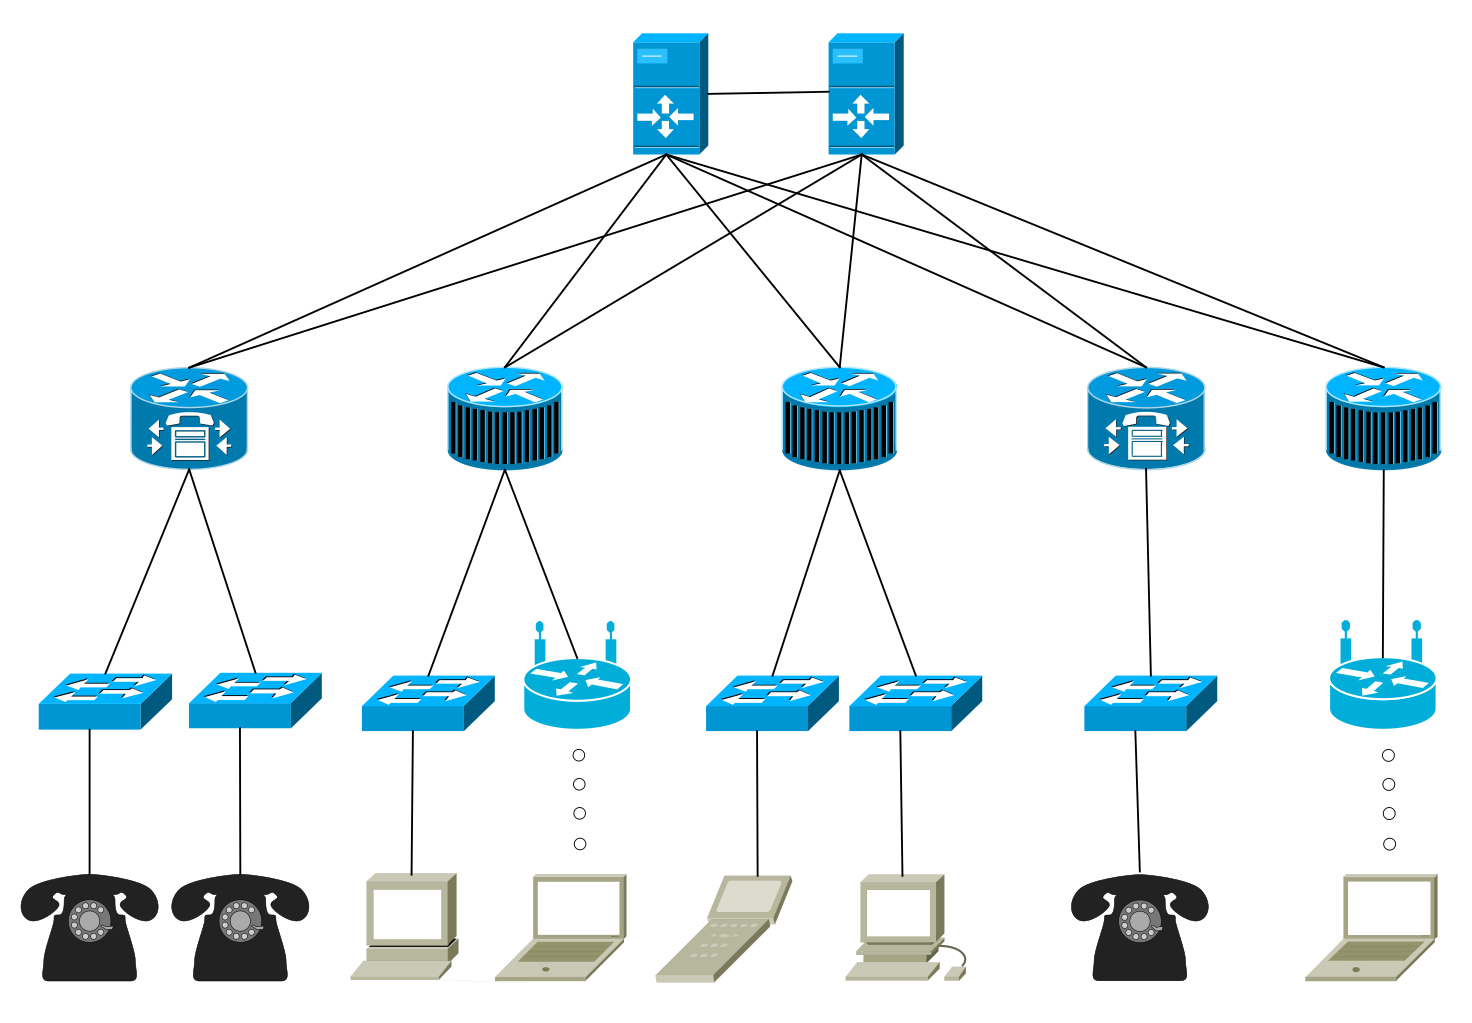
\includegraphics[width=1\textwidth]{./images/schema-logique.png}
    \caption{Schéma logique hiérarchique du réseau}
\end{figure}

%
    \cleardoublepage
%

\subsubsection{Couche coeur}
C'est la couche supérieure.
Son rôle est de relier entre eux les différents segments du réseau, par exemple les sites distants, les LANs ou les étages d'une société.
Dans notre cas le coeur du réseau sera constitué de deux routeurs.

\subsubsection{Couche distribution}
Cette couche consiste à router, filtrer autoriser ou non les paquets.
C'est a ce niveau que nous allons donc crée des VLANs sur les routeurs afin de délimiter l'étendu du réseau.
Nous décidons de faire deux VLAN principaux : VLAN Interne, VLAN Visiteur.

\subsubsection{Couche accès}
Cette couche est la dernière avant de transmettre le paquet à l'hôte.
Elle ne contient que des commutateurs qui permettrons de relayer l'information.

\subsubsection{Couche hôtes}
Il s'y trouve ici les différents types de terminaux .Tels que les terminaux portatifs, les ordinateurs fixes, les appareils médicaux( Scanner, radio etc).

%
    \cleardoublepage
%
%
\subsection{VLANs}

Nous avons décider de séparer le réseau interne avec celui des visiteurs pour une raison de qualité de service.
Le besoin et la sécurité ne sont pas la même entre ses deux réseaux.

%
%
\subsubsection{VLAN interne}

Le VLAN Interne est divisé à l'intérieur en 3 VLANs.

VLAN Données-Interne:
Il regroupe les différents équipements des bureaux administratif, des salles de réunions et de l'accueil.

VLAN VoIP-Interne:
Il regroupe tous les équipements téléphoniques du personnel de l'hôpital, afin d'assurer une qualité de service vis a vis de la communication dans l'hôpital.

VLAN Médical:
Il regroupe tous les équipements médicaux tels que les scanners , IRM et autre machines a usage médicales.
Il y a aussi les informations des patients stocké dans celui-ci.

%
%
\subsubsection{VLAN visiteur}

Le VLAN Visiteur est lui divisé en 2 VLANs.

VLAN Données-Visiteur:
Il regroupe toutes les données qui seront émises par le visiteur a l'aide de son téléphone portable ou tablette par exemple.

VLAN VoIP-Visiteur:
Il regroupe  tous les équipements téléphoniques fixe installer dans les chambres pour les patients.



%
%
\subsection{Plan d'adressage}

    \begin{center}
        \begin{tabular}{|l|l|r|}
          \hline
            Étages  &   VLAN interne    &   Plage d'adresses \\
          \hline
            tous    &   VoIP-Interne    &   10.0.0.0/16 \\
          \hline
            tous    &   Médical         &   10.1.0.0/16 \\
          \hline
            0 à 4   &   Données-Interne &   10.2.0.0/16 \\
          \hline
            2 à 4   &   VoIP-Visiteur   &   10.128.0.0/16 \\
          \hline
            0 à 4   &  Données-Visiteur &   10.129.0.0/16 \\
          \hline
        \end{tabular}
    \end{center}

%
%
